\documentclass[12pt]{article}
 
\usepackage[margin=1in]{geometry}
\usepackage{amsmath,amsthm,amssymb}
\usepackage{graphicx}
\usepackage{float}

\begin{document}
 
\title{\textbf{Homework 2}}
\author{Fubang ZHAO\\ 
fubang.zhao@polytechnique.edu}
 
\maketitle

\section*{MAP estimation on NMF}
Given the following probabilistic non-negative matrix factorization (NMF) model: (for f = 1, . . . , F , n = 1, . . . , N , k = 1,...,K)
\begin{align*}
w_{f,k} & \sim \mathcal{G} (w_{f,k};\alpha_w, \beta_w ) \\
h_{k,n} & \sim \mathcal{G} (h_{k,n}; \alpha_h, \beta_h ) \\
v_{f,n}|w_{f,:},h_{:,n} &\sim \mathcal{PO} (v_{f,n}; \sum_{k=1}^K{w_{f,k} h_{k,n}})
\end{align*}
where $\mathcal{G}$ and $\mathcal{PO}$ denote the gamma and the Poisson distributions, respectively.

\section*{Question 1}
Derive an Expectation-Maximization algorithm for finding the maximum a-posteriori estimate (MAP), defined as follows:
\begin{equation}
(W^*, H^*) = \underset{W,H}{argmax} \log p(W, H|V)
\end{equation}

Here, we define a latent random variable:
\begin{equation}
s_{f,k,n} \sim \mathcal{PO}(s_{f,k,n}; w_{f,k} h_{k,n}), \quad v_{f,n}=\sum_k s_{f,k,n}
\end{equation}
Then we will transform the problem by introducing $S = [s_{fkn}]_{f,k,n}$:
\begin{align*}
(W^*, H^*) &= \underset{W,H}{argmax} \log p(W, H|V) \\
&= \underset{W,H}{argmax} \log \frac{p(V|W,H)p(W,H)}{p(V)}\\
&= \underset{W,H}{argmax} \log p(V|W,H)p(W,H) \\
&= \underset{W,H}{argmax} \sum_S \log p(V,S|W,H) + \log p(W,H) \\
&= \underset{W,H}{argmax} \sum_S \log p(V|S)p(S|W,H) + \log p(W,H)
\end{align*}
And $v = s_1 + s_2 + ... + s_K$, then:
\begin{align*}
\log p(V|W, H) &= \log \sum_S p(V|S)p(S|W,H) \\
& = \log \prod_{f,n} \mathcal{PO}(v_{f,n};\sum_k w_{f,k}h_{k,n}) \\
&= \sum_f \sum_n(v_{f,n} \log[WH]_{f,n} - [WH]_{f,n} - \log \Gamma(v_{f,n}+1))
\end{align*}
Then, according to the Jensen's inequality, we define:
\begin{align*}
\mathcal{L}_V(W, H)&=\log \sum_S p(V|S)p(S|W,H) \\
&\geq \sum_S q(S) \log \frac{p(V,S|W,H)}{q(S)} \\
&=\mathcal{B}_{EM}[q]
\end{align*}
To make the bound tight for a particular value of $\theta$, we need for the step involving Jensen’s inequality in our derivation above to hold with equality. For this to be true, we know it is sufficient that that the expectation be taken over a “constant”-valued random variable. It means:
\begin{equation}
q(S) \propto p(V,S|W,H)
\end{equation}
Since we know that $\sum q(S) = 1$, we can get that:
\begin{align*} 
\underset{q(S)}{argmax} \mathcal{B}_{EM}[q]&= \frac{p(V,S|W,H)}{\sum_S p(V,S|W,H)} \\
&= \frac{p(V,S|W,H)}{p(V|W,H)} \\
&= p(S|V,W,H)
\end{align*}
Here,  
\begin{align*}
\underset{W,H}{argmax} \mathcal{B}_{EM} &= \underset{W,H}{argmax}\sum_S q(S) \log \frac{p(V,S|W,H)}{q(S)} \\
&= \underset{W,H}{argmax} \sum_S q(S) \log p(V,S|W,H) \\
&= \underset{W,H}{argmax} \mathbb{E}[logp(V,S|W,H)]_{q(S)^{(n)}}
\end{align*}
Hence the problem can be maximized iteratively as follows:
\begin{align*}
&E\;step \quad q(S)^{(n)} = p(S|V, W^{n-1}, H^{n-1}) \\
&M\;step \quad (W^{n}, H^{n}) = \underset{W,H}{argmax} \mathbb{E}[logp(V,S|W,H)]_{q(S)^{(n)}} + \log p(W,H)
\end{align*}

\subsubsection*{The E Step} To derive the posterior of the latent sources, we observe that
\begin{equation}
p(S|V,W,H) = \frac{p(V,S|W,H)}{p(V|W,H)}
\end{equation}
For this model, we can get:
\begin{align*}
& \log p(V,S|W,H) \\
& \qquad  = \sum_f \sum_n\left(\sum_k(-w_{f,k}h_{k,n}+s_{f,k,n}\log (w_{f,k}h_{k,n})-log\Gamma (s_{f,k,n}+1)+\log \delta(v_{f,n}-\sum_k s_{f,k,n}))\right)
\end{align*}
According to (4), we can get:
\begin{align*}
&\log p(S|V,W,H) \\
&\qquad = \sum_f \sum_n\left(\sum_k (s_{f,k,n}log\frac{w_{f,k}h_{k,n}}{\sum_{k'} w_{f,k'}h_{k',n}} - log\Gamma(s_{f,k,n} + 1) + log\;\Gamma(v_{f,n} + 1) +log\delta (v_{f,n} - \sum_k s_{f,k,n}))\right) \\
&\qquad = \sum_f \sum_n log\;\mathcal{M}(s_{f,1,n},...s_{f,K,n};v_{f,n}, p_{f,1,n},...,p_{f,K,n})
\end{align*}
where $p_{f,k,n} = w_{f,k}h_{k,n} / \sum_{k'} w_{f,k'}h_{k',n}$ are the cell probabilities. Here, $\mathcal{M}$ denotes a \textbf{multinomial distribution} defined by
\begin{align*}
\mathcal{M}(\textbf{s};v;\textbf{p})
&=\begin{pmatrix}v \\s_1s_2\cdots s_K\end{pmatrix} p_1^{s_1}p_2^{s_2}\cdots p_K^{s_K}\delta(v - \sum_k s_k) \\
&= \delta(v - \sum_k s_k)v!\prod_{k=1}^K\frac{p_k^{s_k}}{s_k!}
\end{align*}
According to the definition of  multinomial distribution, we can get the marginal mean:
\begin{equation}
\mathbb{E}[s_k] = v p_k
\end{equation}

\subsubsection*{The M Step}

We know that the Gamma distribution is
\begin{equation}
\log \mathcal{G}(x;\alpha, \beta) = (\alpha -1) \log x - \frac{x}{\beta} - \log \Gamma (\alpha) -\alpha \log \beta
\end{equation}
And because W and H are independent, $\log p(W,H) = \log p(W) + \log p(H)$

\begin{align*}
	&\mathbb{E}[log p(V,S|W,H)]_{q(S)^{(n)}} + \log p(W,H) \\
	&= \sum_f \sum_n \left( \sum_k (-w_{f,k}h_{k,n}+\mathbb{E}[s_{f,k,n}]log(w_{f,k}h_{k,n}) - log\Gamma(\mathbb{E}[s_{f,k,n}] + 1) + log\delta (v_{f,n} - \sum_k \mathbb{E}[s_{f,k,n}])) \right) \\
	&+  \sum_f\sum_k\left((\alpha_w - 1)\; log\; w_{f,k} - \frac{w_{f,k}}{\beta_w} - \Gamma(\alpha_w) - \alpha_w\;log(\beta_w)\right) \\
	&+ \sum_n\sum_k\left((\alpha_h - 1)\; log\; h_{k,n} - \frac{h_{k,n}}{\beta_h} - \Gamma(\alpha_h) - \alpha_h\;log(\beta_h)\right)
\end{align*} 
where $\mathbb{E}[s_{f,k,n}] = v_{f,n}p_{f,k,n}$, and we only need to maximize the simpler objective:
\begin{align*}
	\mathcal{L}(W,H) &= \sum_f \sum_n\left(\sum_k (-w_{f,k}h_{k,n}+\mathbb{E}[s_{f,k,n}]log(w_{f,k}h_{k,n}))\right)\\
	&+  \sum_f\sum_k\left((\alpha_w - 1)\; log\; w_{f,k} - \frac{w_{f,k}}{\beta_w})\right) \\
	&+ \sum_n\sum_k\left((\alpha_h - 1)\; log\; h_{k,n} - \frac{h_{k,n}}{\beta_h})\right)
\end{align*}

and the solution is given by the following equations
\begin{align*}
	\frac{\partial \mathcal{L}}{\partial w_{f,k}} &= -\sum_n h_{k,n}^{i} + \frac{\sum_n \mathbb{E}[s_{f,k,n}^{i}] + (\alpha_w - 1)}{w_{f,k}} - \frac{1}{\beta_w} \\
	w_{f,k}^{i+1} &=  \frac{w_{f,k}^i \sum_n \frac{v_{f,n}h_{k,n}^i}{\sum_{k'} w_{f,k'}^i h_{k',n}^i} + (\alpha_w - 1)}{1/\beta_w +  \sum_n h_{k,n}^i}\\
	\frac{\partial \mathcal{L}}{\partial h_{k,n}} &= -\sum_f w_{f,k}^{i} + \frac{\sum_f \mathbb{E}[s_{f,k,n}^{i}] + (\alpha_h - 1)}{h_{k,n}} - \frac{1}{\beta_h} \\
	h_{kn}^{i+1} &=  \frac{h_{k,n}^i \sum_f \frac{v_{f,n}w_{f,k}^i}{\sum_{k'} w_{f,k'}^i h_{k',n}^i} + (\alpha_h - 1)}{1/\beta_h + \sum_f w_{f,k}^i}\\
\end{align*}

\section*{Question 2}

1. The code is in the folder with the name $"hw2\_Intro\_graphic.ipynb"$.
\\\\
2. The result is shown below:

\begin{figure}[H]
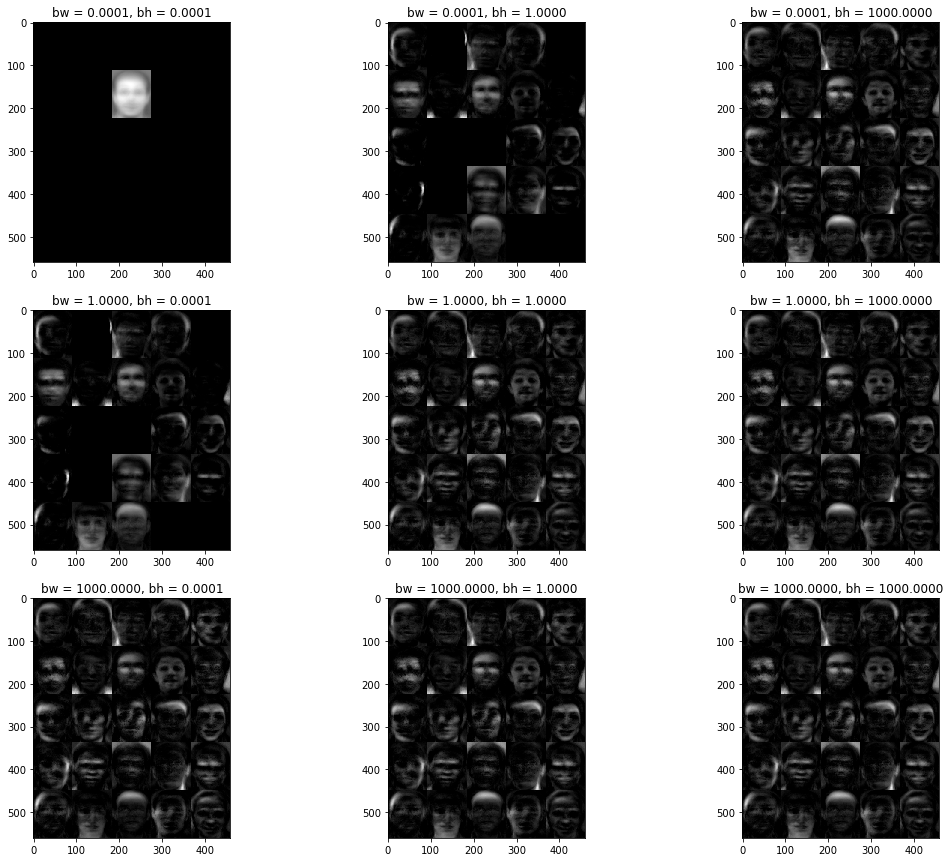
\includegraphics[scale=0.5]{p1} 
\caption{The different W with the changes of aw and ah}\label{fig:1} 
\end{figure}
Here, we set the range of $\beta_w, \beta_h$is: $[0.001,\; 1,\; 1000]$. According to the result, we find that: 
\begin{enumerate}
\item[a.]
when $\beta_w<1\;or\; \beta_h<1$, the characters of faces are not that clear.
\item[b.]
when $\beta_w>=1\;or\; \beta_h>=1$, the differences between the results are very little, and are much clearer than those with smaller $\beta_w, \beta_h$.
\end{enumerate}
3. The result is shown below:
\begin{figure}[H]
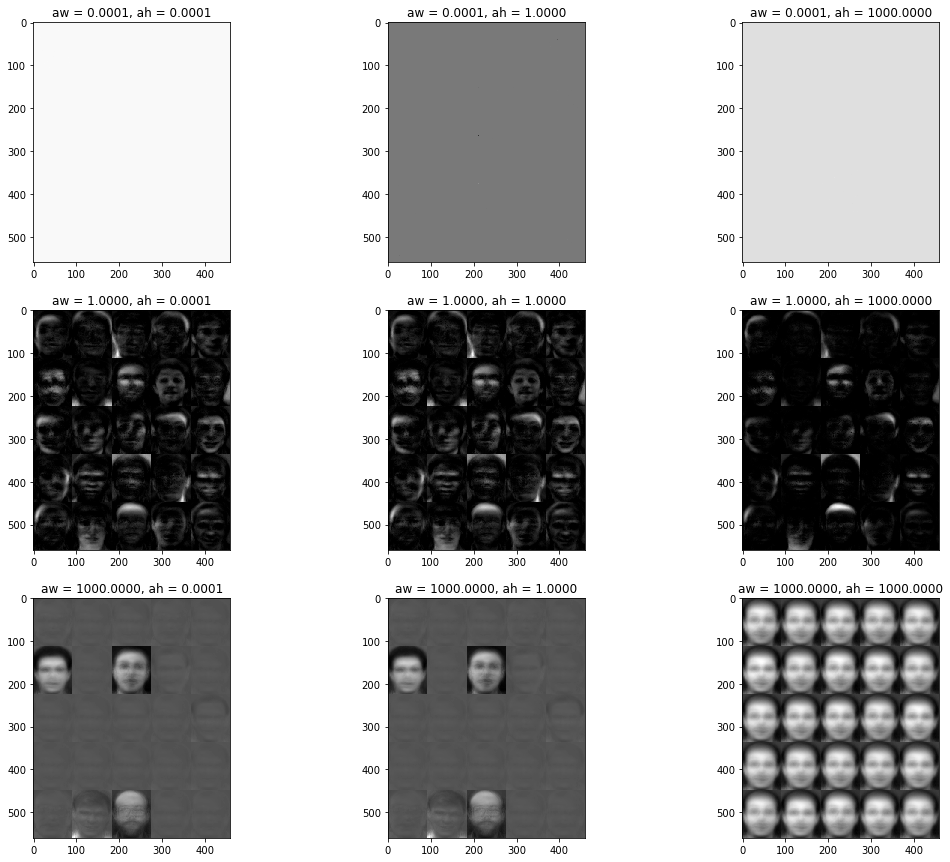
\includegraphics[scale=0.5]{p2} 
\caption{The different W with the changes of bw and bh}\label{fig:2} 
\end{figure}
Here, we set the range of $\alpha_w, \alpha_h$ is: $[0.001,\; 1,\; 1000]$. According to the result, we find that: 
\begin{enumerate}
\item[a.]
when $\alpha_w=0.0001$, the characters of faces almost disappear. It is almost no character left.
\item[b.]
when $\alpha_w=1000$, the characters are also not clear. Especially, when $\alpha_w=\alpha_h=1000$, the 25 faces are almost the same one. 
\item[c.]
When $\alpha_w=\alpha_h=1$, the result is the best. The characters of faces are the most recognizable.
\end{enumerate}

\end{document}
